\section{Proofs to Selected Results}
\label{sec:proofs}

\subsection*{$R(P,\dfw(K)) = \tilde{R}(P,K)$}

The asynchronous semantics under $\dfw(K)$ and the compositional semantic are
equivalent. Figure~\ref{fig:proofs:cs} shows the construction of the interface
\emph{I} that summarizes exactly execution produced by $\dfw(1)$ scheduler
(given in in Figure~\ref{fig:proofs:cs}(a)). Consider Task $A$, that
consequently creates tasks $B$ and $C$, waits for $B$ (at the end of segment 1)
and waits for \emph{C} (at the end of segment 4). $C$ is a delaying task
(delays after segment 3) and completes after segment 5.

Basically, $A$ updates the current state it executes in (following the standard
sequential semantics). Each time it creates a task, it collects and sequences
together the interfaces of these created tasks into $J$ (see the sequencing of
the interfaces of $B$ and $C$ in Figure~\ref{fig:proofs:cs}(b)). When it waits
for a task, it sequences the accumulated tasks in $J$ into $I$ (as in
Figure~\ref{fig:proofs:cs}(c). Then, it continues with its internal execution.
When $A$ waits for the delaying task \emph{C}, $J$ does not keep new posted
tasks to be joined into $I$, hence $I$ is not updated. But $A$ continues
sequencing the rest of its execution (segment 6) in a later round in which $C$
completes. When $A$ completes, it ends up with the interface \emph{I} that
summarizes the execution in Figure~\ref{fig:proofs:cs}(a).

\begin{figure}
  \center
  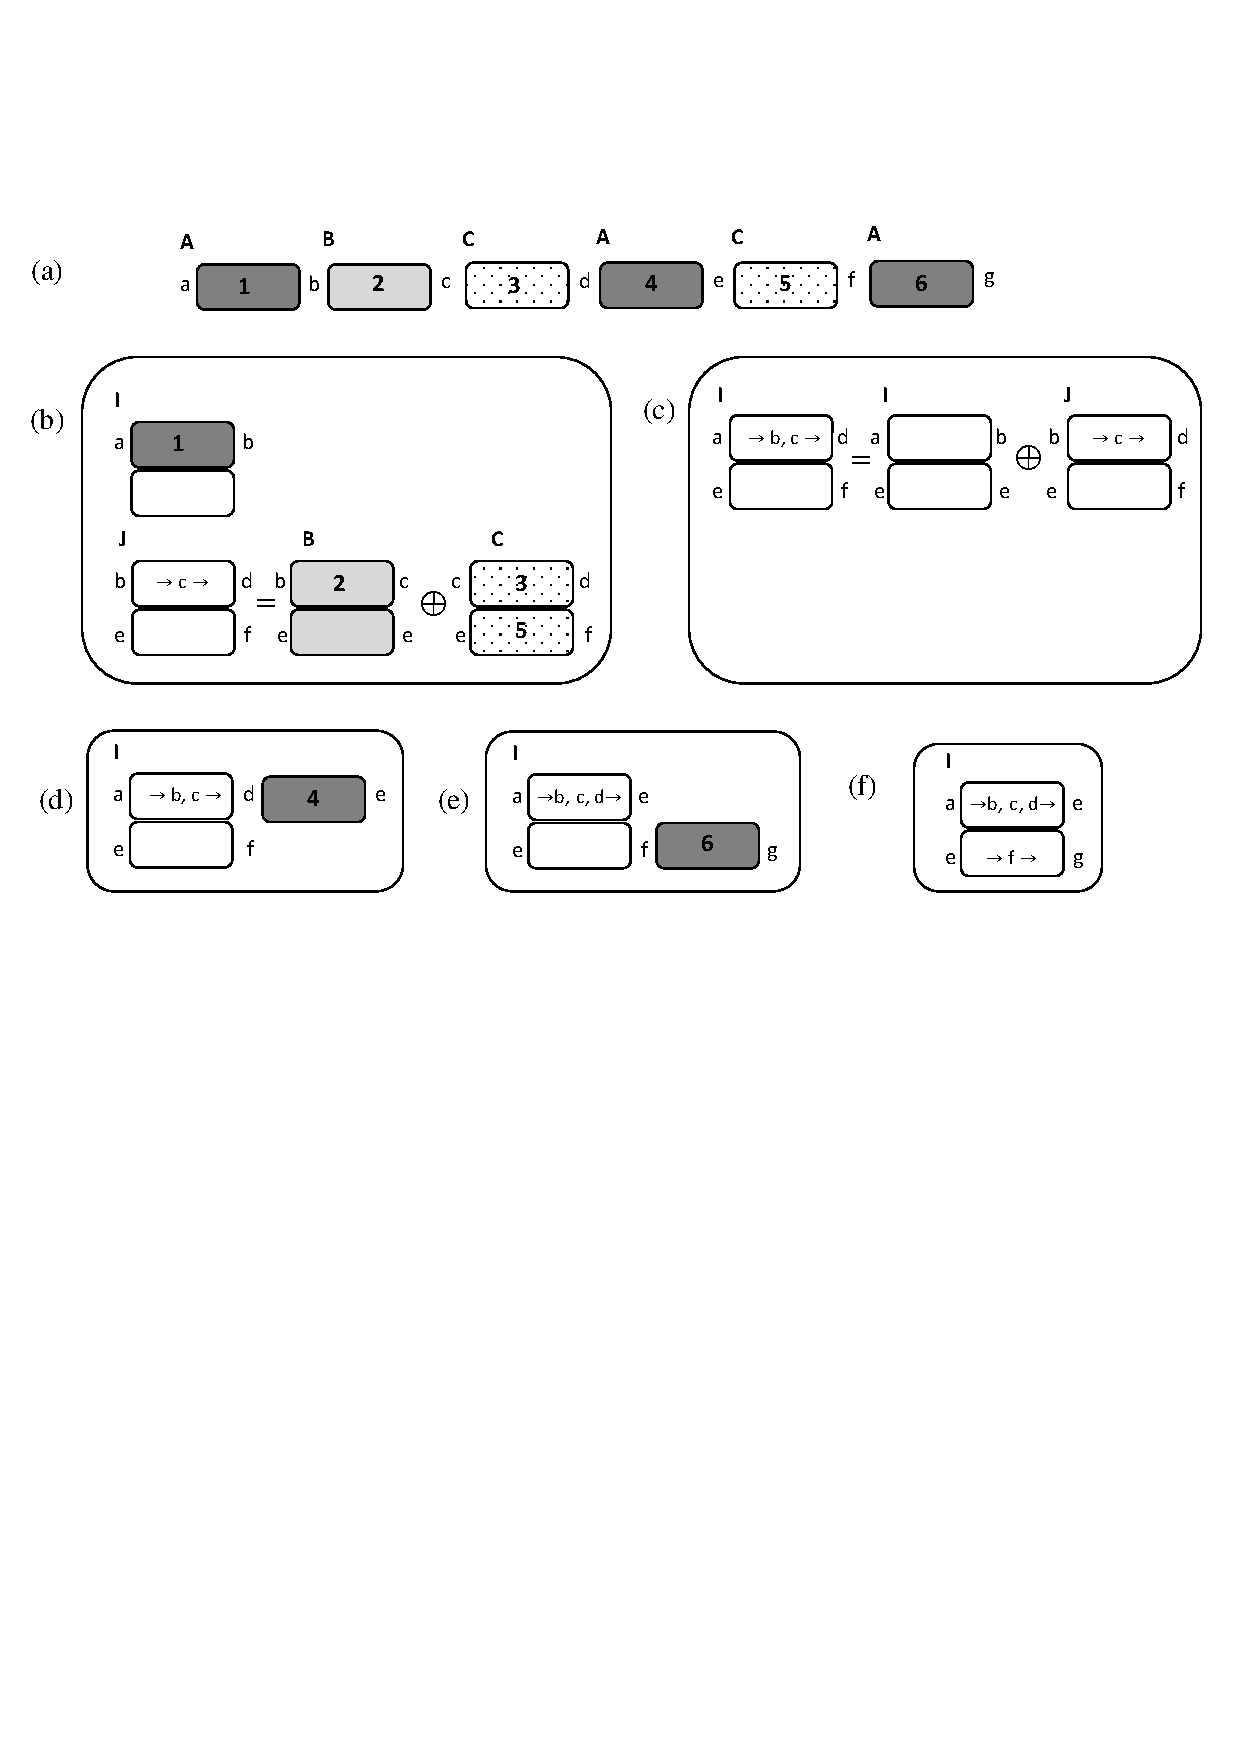
\includegraphics[width=8cm]{figures/figure-cs}
  \caption{Simulating an asynchronous program using compositional semantics.}
  \label{fig:proofs:cs}
\end{figure}

   
We can show the equivalence between the $\dfw(K)$ execution and the
compositional semantics inductively. Consider building the execution of a
program $P$. Initially, $P$ starts in round $0$ with an initial state $g_0$,
having $I[0]\mathsf{.in} = g_0$. At each statement of $P$, the compositional
semantics builds the interface $I$ of $P$ iteratively.

\begin{itemize}

  \item At each execution of a sequential statement, it updates its current
  state $g \rightarrow g'$ yielding $\tup{g, w, k, d, I, J} \rightarrow
  \tup{g', w, k, d, I, J}$.

  \item At each task creation, it creates a new task interface summarizing its
  child task and joins this new child task's interface to the collected tasks.
  The join operation ensures that this new task starts its execution where the
  last posted task has left off. Hence, it simulates the execution of this task
  in the ordering that $\dfw(K)$ provides. As a result of the join operation,
  $\mathsf{out}$ of $J$ now keeps the effects of this last posted task.
  Sequencing an interface of another task to $J$ will simulate that task to
  start from where the last task in $J$ ends in.

  \item When a task waits, the cumulated tasks in $J$ update $I$ by appending
  to it, enabling the next statements of the program to operate on the state
  reached by executing the tasks in $J$. The transition also moves the current
  task to the round and the state where the waited task has completed. This
  simulates the execution under $\dfw(K)$ that schedules the waiting task in
  the round that the waited task completes, after the execution of all its
  children tasks. Notice that the input and the output intermediate states of
  $I$ are equal, since the task waits and does not involve in the execution
  until the waited task completes.

  \item When a task is delayed, {\sc CDelay} assigns the current state to the
  out state of the interface, and moving the next state in a later round.

\end{itemize} 

At the end of the execution, $I[k]\mathsf{.out}$ keeps the state reached in at
most $k$ delays.




\subsection*{$R_{@p}(@S(P,K)) = \tilde{R}(P,K)$}

Here, we prove that for an asynchronous program $P$, our translation precisely
produces the compositional semantics and the set of reachable global values in
the $K$-delay sequentialization $@S(P,K)$ of an asynchronous program $P$ is
precisely equal to the set of values reachable in $P$ in the $K$ bounded
compositional semantics.

Our sequentialization actually encodes the interfaces in the compositional
semantics using {\tt G}, {\tt Guess}, {\tt Next} and {\tt Save} variables.
Essentially, {\tt Next} keeps $J\mathsf{.out}$ and gets updated each time $J$
is joined with a newly posted task. To be able to append the posted tasks after
the internal task that creates them, initially {\tt Next} is set to the state
it pauses (in either a \<wait> or \<return> statement) or delays. Since do not
know that state initially, we guess the ending states of each round and keep in
{\tt Guess}. When we reach to that pause/delay point, we validate the guess.

\begin{itemize}

  \item The {\sc CAsync} rule is encoded by the translation of the \<async>
  statement. The translation sets the current state {\tt g} to the {\tt next}
  state where the last posted task has finished with (corresponding to the
  $J\mathsf{.out}$). It updates the {\tt next} variable with the new task's
  ending state which is guessed before its execution and it is verified to be
  the current state after the execution of the posted task. This precisely
  captures the generation of a new interface for the new task and joining it
  with the accumulated task interface $J$.

  \item {\sc CWait} rule is encoded by the translation of \<wait> statement.
  The translation verifies the guess that keeps the pause state of the current
  task to be the current state and sets the state to {\tt next} that keeps the
  ending state of the last posted task. This has the same behavior with the
  {\sc CWait} rule as it joins the current interface with $J$ (ensuring that
  the out state of the $I$ is equal to the in state of $J$). Since the
  translation does not touch the states {\tt g[i]} in the intermediate rounds,
  it satisfies the equality of the $\mathsf{in}$ and $\mathsf{in}$ states of
  these intermediate rounds.

  \item {\sc CDelay} rule is encoded in the translation of preemption that
  increases the current round. Since the program reads the value of the {\tt g}
  as {\tt g[i]} in a given round $i$, it already operates on the state
  corresponding to its current round.

\end{itemize}  

\subsection*{The $\dfw(K)$ value reachability problem is in NP.}

We prove membership in NP by constructing a polynomial time algorithm that
verifies a polynomial-sized execution witness in polynomial time. The
algorithm reaches its final state iff the provided witness represents a valid $\dfw(K)$ execution of a given program $P$, hence reduces our NP-membership problem to the reachability in this verifier program.

For this aim, we define (i) a witness that represents an $\dfw(K)$ execution of a given program $P$ in polynomial size, and (ii) construct a polynomial time algorithm to verify a witness by a translation from tasks' codes.  As distinct from our $DFW(k)$ translation that uses $O(K)$ number of variables (keeping $K$ copies of global variables) that yield an exponential number of valuations, we need to build an $O(1)$ translation to conform with the polynomial-time requirement. 

We define a witness as a list of task interfaces which are preempted/delayed at least once throughout its execution (which we will refer to a "delaying task"), ordered in the depth-first traversal order of the task creation tree of $P$. The size of the list (as well as the integer variables used in the translation) is bounded to $K$ due to the delay bound $K$.  

A task interface summarizes the execution of a task together with the execution of the tasks it creates (its children tasks). In other words, the execution in between $g\mathsf{.in}[R]$ and $g\mathsf{.out}[R]$ states of a round $R$, encapsulates both the parent and the children tasks' execution in that round. In addition to the $g\mathsf{.in}$ and $g\mathsf{.out}$ states of each round, task interface keeps the number of children of that task and their indices in their appearance order in the witness, necessary for its verification.     

The verifier program (main procedure in Figure~\ref{fig:comp:NP}), having multiple assume statements enforce the task interfaces to be sequenced in the $\dfw(K)$ order. It completes its execution iff the task interfaces in the witness provide a valid execution when sequenced in that order. 

The task interfaces are verified one by one by checking whether the execution of this task yields the $g\mathsf{.in}$ and $g\mathsf{.out}$ states of its interface and it posts all its children tasks in the given order. A major challenge is to check all rounds of a task and its children tasks in a single call to a task's procedure, without keeping copies of global variables for each round. To overcome this, we use the facts that (i) we already have the $g\mathsf{.in}$ and $g\mathsf{.out}$ states of all rounds of the delaying tasks in the witness and (ii) non-delaying tasks complete in the current round being simulated. We verify a task interface by simulating the execution of that task starting from the $g\mathsf{.in}$ of the initial round of a task and during that time we cumulate the effects of the children at task creation points. We use {\tt next} to keep the state in which next task will start with, initially the state where the current task waits, gets delayed (preempts) or returns (at a state where it pauses/completes its execution). The idea is to update {\tt next} using the children interfaces (so that next keeps the effects of tasks to-be-executed at a pause/return point) and updating the current state {\tt g} using calculated {\tt next} state. Since the parent task does not involve in the rounds later than its completion round, these rounds of the interface are verified by only matching the $g\mathsf{.in}$ and $g\mathsf{.out}$ states of the children tasks.

\begin{figure*}[t]
\centering
  \begin{minipage}[t]{8.5cm}
    \lstset{language=program}
    \lstset{basicstyle=\ttfamily\scriptsize}
    \begin{lstlisting} 
TaskInterface{
	start: K // round the task starts $\in$ {0,1,..K}
	end: K // round it ends
	val: G // return value
	proc: Proc x E
	gin, gout: G^K
	numChildren: K 
	children: K^numChildren 
}

// Globals:
var	tasks: TaskInterface;
var	K: int; // max # of delays
var R: // current round being simulated
var this: TaskInterface; // currently simulated task
var numPosted: K; // current # of children of "this"
// # of children scheduled before "this"
var childrenBeforeMe: K; 
var g, next, guess: G

proc main(witness: TaskInterface^K)
	tasks := witness;
	for i=0 to K-1
		this = tasks[i];
		R := tasks[i].start; 
		g := tasks[i].gin[R];
		numPosted := 0;
		childrenBeforeMe := 0;
		next := guess := *;
		
		call (this.proc)'; // call the translation of proc
		
		assume guess = g; 
		
		//verify the interface
		assume numPosted = this.numChildren;
		assume this.end = R;

		// continue the round with the next children
		for i=childrenBeforeMe to numChildren-1
			assume next = tasks[this.children[i]].gin[R]; 
			next := tasks[this.children[i]].gout[R];
		end;

		// end round R
		assume this.gout[R] = next;

		// simulate next rounds of my children
		if numPosted > 0
			while R < K-1
				R++;
				assume this.gin[R] = 
					tasks[this.children[0]].gin[R];
				for i=0 to this.numChildren-1
					assume tasks[this.children[i]].gout[R] =  
						tasks[this.children[i+1]].gin[R];
				end;
			end;
		end;
			
		// end last round
		assume this.gout[R] = 
			tasks[this.numChildren-1].gout[R];
	end;
end


// translation of a procedure p(e) s
proc p(e) 
	var save: G * G;	
	s'; // translation of s
end
      \end{lstlisting}
    \end{minipage}
 %   \hfill
    \begin{minipage}[t]{8.5cm}
      \lstset{language=program}
      \lstset{basicstyle=\ttfamily\scriptsize}
      \begin{lstlisting}
// translation of async t := p e
if * && <p,e> =  this.children[numPosted].proc 
&& R = tasks[numPosted].start then
	assume next = tasks[numPosted].gin[R]; 
	next := tasks[numPosted].gout[R];
	// set the value and the end round of t
	t := (tasks[numPosted].val, tasks[numPosted].end);
	numPosted ++;
else  // posted task is not a delaying task
	save := <g, guess>;  g := next;
	guess := next := *;
	call x := p e;   // will complete in the current round
	// set the value and the end round of t
	t := (x, R);
	assume guess = g;  <g, guess> := save;
end;


// translation of x := wait t:
x, t_end := t;

if t_end > R
	// if t completes in a later round
	// this round ends in "next"	
	assume this.gout[R] = next; 
end;

if numPosted > 0 
	// simulate children rounds up to t_end
	while R < t_end
		R++;
		assume this.gin[R] = tasks[this.children[0]].gin[R];
		for i=0 to numPosted - 1
			assume tasks[this.children[i]].gout[R] = 
				tasks[this.children[i+1]].gin[R];
		end;		
		assume this.gout[R] = 
			tasks[this.children[numPosted-1]].gout[R];
	end;

	//simulate children in round R=t_end and set next
	next = tasks[this.children[0]].gin[R];
	for i=0 to numPosted -1
		assume next = tasks[this.children[i]].gin[R];
		next := tasks[this.children[i]].gout[R];
	end;
end;

// update g and next
assume guess = g;  
g := next;	
next := guess := *; 
	
childrenBeforeMe := numPosted;


// translation of preemption:
assume guess = g;  

// simulate the children in the current round
for i=childrenBeforeMe to numPosted - 1
	assume next = tasks[this.children[i]].gin[R];
	next := tasks[this.children[i]].gout[R];
end;

// end current round
assume this.gout[R] := next;
R++;

// simulate the children before me
if childrenBeforeMe > 0 then
	assume this.gin[R] = tasks[this.children[0]].gin[R];
	for i=0 to childrenBeforeMe - 2
		assume tasks[this.children[i]].gout[R] 
			=  tasks[this.children[i+1]].gin[R];
	end;
end;

// current state is where the children leaves off
g := tasks[this.children[i]].gout[R]; 
next := guess := *; 
    \end{lstlisting}
  \end{minipage}
  \caption{Translation to construct the verifier program}
  \label{fig:comp:NP}
\end{figure*}


